\section{Planare Rekonstruktion} \label{sec:plane-reconstruction}

Dieses Kapitel widmet sich der Idee, eine Rekonstruktion für ein Rekonstruktions basiertes Überlagerungsverfahren durch eine Ebenendetektion zu realisieren. \citet{yang2010plane} erwähnt hierzu, dass Ebenen in fast allen künstlichen Umgebungen zu finden sind und auf Grund ihrer vorteilhaften geometrischen Eingenschaften in verschiedensten Computer Vision Verfahren verwendet werden. Daher gibt es viele Forschungsarbeiten, Methoden und Algorithmen, um aus verschiedensten Informationsquellen ein Ebenenmodell zu extrahieren.

Das \enquote{Simultaneous Localization and Mapping} (SLAM) Verfahren von \citet{trevor2012planar} detektiert Ebenen mit dem RANSAC Algorithmus. RANSAC bietet gegenüber anderen Algorithmen zur Ebenen Detektion den Vorteil, ein Modell auch bei vielen Ausreißern performant zu ermitteln. Agglomeratives Clustering und Region Growing wie von \citet{feng2014fast} beschreiben, eignet sich auf Grund des Ausgabeformats von Project Tango nicht direkt, da es keine organisierte Point Cloud ausgibt und die Daten durch Reflektionen und Löchern stärker mit Fehlern behaftet sind. 

Das selbst zusammengestellte Verfahren zur Ebenendetektion besteht daher aus folgenden Komponenten. Wie in dem Ansatz von \citet{yang2010plane} wird der RANSAC Algorithmus auf Würfeln ausgeführt, die eine Menge gesammelter Punkte aus der Pointcloud beinhaltet. Dabei entsprechen die Würfel den untersten Knoten eines Octrees, welcher hier zur Speicherung und Aufnahme aller Punkte verwendet wird. Diese untersten Knoten des Octrees werden folgend auch Cluster genannt. Eine gefundene Ebene in einem Würfel wird wie im SLAM Verfahren von \citet{trevor2012planar} persistiert. Die Repräsentation der Ebene \(P\) wird dort wie in Gleichung \ref{eq:plane} festgehalten. Dabei handelt es sich um den Normalenvektor \(\vec{n}\) und der Distanz zum Ursprung \(d\) der Hesse Normalform einer Ebene, sowie der Punkte der konvexen Hülle \(H\). \citet{trevor2012planar} erläutern, dass die konvexe Hülle in der Repräsentation festgehalten wird, um eine sukzessive Verbesserung einer Ebene nach mehreren Messdurchläufen zu ermöglichen. So werden die Punkte der konvexen Hülle pro Messvorgang kombiniert, damit die Ebenenausbreitung auch außerhalb des Sichtfeldes beibehalten werden kann. 

\begin{equation} \label{eq:plane}
P=\left[\vec{n}, d, H\right] \qquad H=\vec{h_1}, \vec{h_2}, \ldots  \vec{h_n}
\end{equation}

Die einzelnen Schritte des Vorgehens werden in den folgenden Absätzen näher erläutert. Ein grober Ablauf des Vorgehens wird aber bereits in Listing \ref{lst:planeReconstruction} zusammengefasst und in Pseudocode beschreiben. 

\begin{lstlisting}[mathescape,caption=Planare Echtzeit Rekonstruktion, label=lst:planeReconstruction, float=htbp]

Eingabe: Octree $O$, Anzahl der zu suchenden Ebene in Clustern $N$
Ausgabe: Polygonpunkte $T_{Gesamt}$

für jedes Cluster $C$=[$C_{Punkte}$, $C_{Ebenen}$] aus $O$
    führe $N$ mal aus
        bestimme Ebene [$\vec{n}$, $d$, $P$] mit RANSAC aus $C_{Punkte}$
        wenn keine Ebene mit genügend $P$ gefunden wurde
            nächstes Cluster (continue)
        wenn Ebene mit [$\vec{n}$, $d$, $H_{alt}$] in $C_{Ebenen}$ existiert	
            füge die konvexe Hülle $H_{alt}$ zu $P$ hinzu	
        bestimme die konvexe Hülle $H_{neu}$
        trianguliere $H_{neu}$ zu $T_{Ebene}$
        $T_{Gesamt}$ += $T_{Ebene}$
        $C_{Ebenen}$ += [$\vec{n}$, $d$, $H_{neu}$]
        $C_{Punkte}$ - $P$
\end{lstlisting}


\subsection{RANSAC zur Ebenendetektion} \label{sec:ransac}

Um mit dem RANSAC Algorithmus, beschrieben in Kapitel \ref{sec:ransac-theory}, Ebenen in einer Punktewolke bestimmen zu können, werden pro Iteration drei Stichproben \(\vec{A}\), \(\vec{B}\) und \(\vec{C}\) gewählt, die zur Bestimmung einer Ebene ausreichen. Das Ebenenmodell, hier in der Hesse Normalform mit dem Normalenvektor \(\vec{n}\) und dem Abstand zum Koordinatenursprung \(d\), lässt sich dabei durch die Gleichung \ref{eq:normalform} bestimmen.

\begin{equation}\label{eq:normalform}
\vec{n} =\left|\left| \vec{AB} \times \vec{AC}\right|\right|
\qquad
d = \vec{A} \cdot \vec{n}
\end{equation}

Um zu ermitteln ob ein Punkt \(\vec{P}\) aus einer Messreihe die gefundene Ebene \(\left[\vec{n}, d\right]\) unterstützt, wird die kürzeste Distanz \(d_P\) zwischen Punkt und Ebene wie in Gleichung \ref{eq:plane-distance} ermittelt.  Ein entsprechender Toleranzwert für die Distanz \(d_{min}\), im gezeigten RANSAC Algorithmus \(e\) genannt, wird später bei der Umsetzung abhängig von der Ungenauigkeit des Tiefensensors gewählt. 

\begin{equation} \label{eq:plane-distance}
d_P = \vec{n} \cdot \vec{P} - d \qquad support_{d_P} = d_P < d_{min}
\end{equation}

Um das finale Modell der Ebene zu bestimmen, wie im ursprünglichen RANSAC Algorithmus in Punkt 7. beschrieben, und somit die Varianz des Abstands der Punkte zur Ebene zu minimieren, wird mit Hilfe der unterstützenden Punkte \(P_{s}=\left[x,y,z\right]\) eine lineare Regression durchgeführt. Diese Mittelt ein Ebenenmodell \(E=\left[\vec{n}, d\right]\) aus den zuvor ermittelten Punkten mit Hilfe der Methode der kleinsten Quadrate. \citet{hoppe1992surface} nutzen dazu für eine ähnliche Problemstellung die Eigenwert Dekomposition der Kovarianzmatrix der Punkte \(P_{s}\) zum Zentrum \(\vec{p_{c}}\). In Gleichung \ref{eq:centroid} wird das Zentrum aus den unterstützenden Punkten \(P_{s}\) bestimmt. Gleichung \ref{eq:covarianz} zeigt die Bestimmung der Kovarianzmatrix \(CV\) im Bezug zum Zentroid, in der \(\otimes\) für das dyadische Produkt\footnote{Wenn \(\vec{a}\) und \(\vec{b}\) die Komponenten \(a_i\) und \(b_j\) beinhalten, resultiert aus \(\vec{a} \otimes \vec{b}\) eine Matrix mit den Komponenten \(a_ib_j\) an der \(ij\) Position. \citep{hoppe1992surface}} steht.

\begin{equation} \label{eq:centroid}
\vec{p_{c}} = \frac{\sum_{n=0}^{|P|} P_{n}}{|P|}
\end{equation}

\begin{equation} \label{eq:covarianz}
CV = \sum_{n=0}^{|P|} ( \vec{p_{n}}- \vec{p_{c}}) \otimes ( \vec{p_{n}}- \vec{p_{c}})
\end{equation}

Wendet man nun auf der Kovarianzmatrix \(CV\) die Eigenwert Dekomposition an, erhält man die Normale \(\vec{n}\) aus dem Eigenvektor \(||\vec{v_i}||\) mit dem kleinsten Eigenwert \(\lambda_i\). Somit würde bei \(\lambda_1 \geqq \lambda_2 \geqq \lambda_3\) die Zuweisung \(\vec{n} = ||\vec{v_3}||\) folgen. Die Distanz zum Ursprung \(d\) entspricht dem Kreuzprodukt aus dem Zentroiden \(\vec{p_c}\) und der neu gewonnen Normalen \(\vec{n}\). \citep{hoppe1992surface} 

\subsection{Bestimmung der Ebenenausbreitung}

Nachdem die Ebene und die korrespondierenden Punkte zur Ebene gefunden wurden, muss noch die Ausbreitung der Fläche bestimmt werden, da die Ebene in Hesse Normalform lediglich die Position \(\vec{n} * d\) und Ausrichtung \(\vec{n}\) festhält. \citet{PlanarSurfaceMapping} nutzt hierfür die konvexe Hülle der korrespondierenden Punkte und trianguliert diese. Wie diese dort genau bestimmt wurde ist nicht beschrieben. 

Um diese Bestimmung performant umsetzen zu können, kann man sich die Eigenschaft der Ebene zu Nutzen machen und die dreidimensionalen Punkte durch Parallelprojektion als zweidimensionale Punkte auf die gefundene Ebene projizieren. Denn die Triangulation ist nach dem Erhalten der zweidimensionalen konvexen Hülle, wie im Listing \ref{lst:triangulation} beschrieben, direkt bestimmbar. Nach der Triangulation können die Ecken der gefundenen Polygone jeweils zurück projiziert werden. Die Gleichungen \ref{eq:projection2d} und \ref{eq:projection3d} bilden die Projektion der Punkte wobei \(R_{\vec{n} \rightarrow \vec{z}}\) der Rotationsmatrix zwischen dem Normalenvektor \(\vec{n}\) und der Z-Achse \(\vec{z}\) entspricht.

\begin{equation} \label{eq:projection2d}
p_{2d} = (p_{3d} - (\vec{n}*d)) * R_{\vec{n} \rightarrow \vec{z}}
\end{equation}
\begin{equation} \label{eq:projection3d}
p_{3d} = (p_{2d} * R_{\vec{n} \rightarrow \vec{z}}^{-1}) + (\vec{n}*d)
\end{equation}

In Abbildung \ref{fig:polygon-process} ist der Gesamtprozess für die Bestimmung der Ebenenausbreitung veranschaulicht. Nachdem eine Ebene mit RANSAC detektiert wurde werden die korrespondierenden Punkte auf diese zweidimensionale Ebene projiziert. Daraufhin wird die konvexe Hülle gebildet und die Triangulation der Hülle bestimmt. Diese Polygon Eckpunkte werden danach wieder zurück in den dreidimensionalen Raum projiziert.

\begin{lstlisting}[mathescape,caption=Bestimmung der Ebenenausbreitung und Triangulation, label=lst:triangulation, float=htb]

Eingabe: Unterstützende Ebenenpunkte aus RANSAC $P$
         Transformation $R_{\vec{n} \rightarrow \vec{z}}$
Ausgabe: Polygone $T_{Ebene}$

    Projiziere alle Punkte aus $P_s$ mit $R_{\vec{n} \rightarrow \vec{z}}$ zu $P_{2d}$
    Bestimme die konvexe Hülle $H$ aus $P_{2d}$ mit Graham Scan
    starte mit leerer Menge $P_{2dmesh}$
    für $i$ von $0$ bis $|H| - 2$
        füge $H_0$ zu $P_{2dmesh}$ hinzu
        füge $H_{i+1}$ zu $P_{2dmesh}$ hinzu
        füge $H_{i+2}$ zu $P_{2dmesh}$ hinzu
    Projiziere alle Punkte aus $P_{2dmesh}$ mit $R_{\vec{n} \rightarrow \vec{z}}^{-1}$ zu $P_{3dmesh}$   
\end{lstlisting}

\begin{figure}[h]
  \centering
	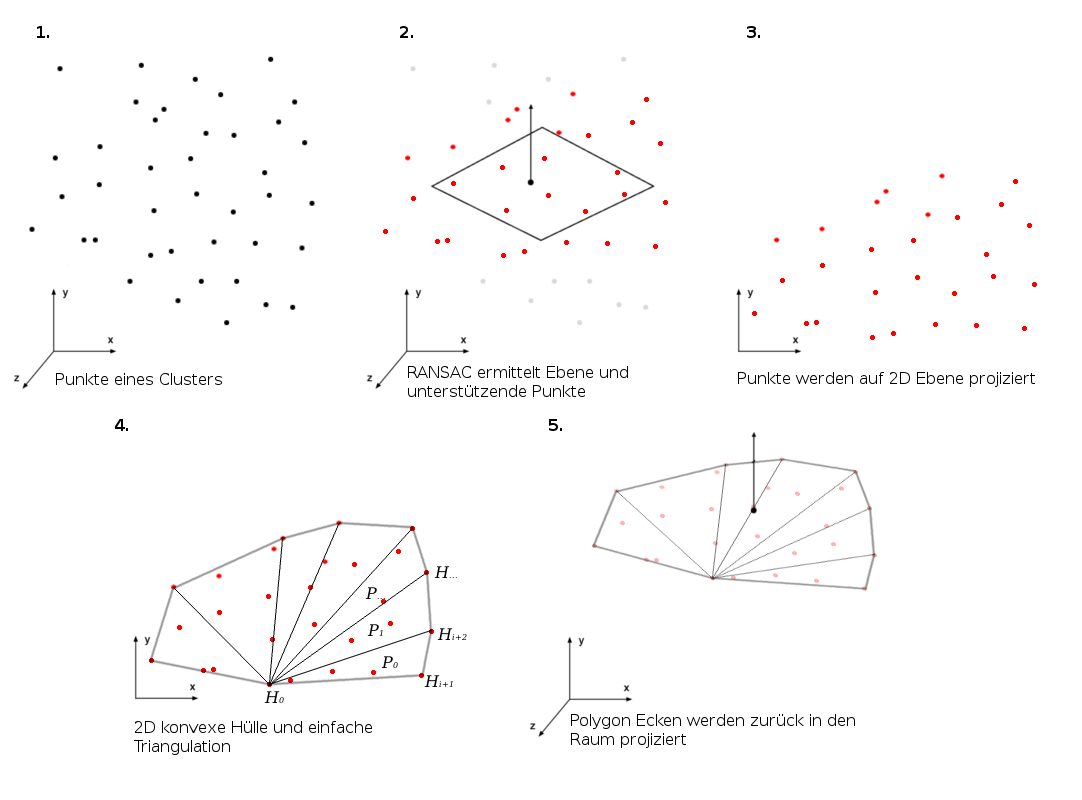
\includegraphics[width=1.1\textwidth]{content/images/methods/polygon-process.png} 
  \caption{Veranschaulichung des Gesamtprozesses zur Bestimmung der Ebenenausbreitung durch RANSAC und der konvexen Hülle.}
  \label{fig:polygon-process}
\end{figure}

\newpage

\subsection{Clustering der aufgenommenen Punkte} \label{sec:cluster}

Wie im Listing \ref{lst:planeReconstruction} zu erkennen wird das zuvor beschriebene Vorgehen für die planare Rekonstruktion immer pro Cluster eines Cluster-Pools durchgeführt. Dadurch werden pro Durchgang des Algorithmus nur ein Bruchteil der gesammelten Punkte rekonstruiert, was wiederum eine Rekonstruktion in Echtzeit möglich macht. Außerdem verhindert das Clustering das Bilden von konvexen Hüllen über Ebenen, die in Zwischenbereichen nicht mit genügend Punkten unterstützt werden. Dieses Problem ist in Abbildung \ref{fig:clustering} links zu sehen, in welcher eine blaue Ebene Rekonstruiert wird, die sich über einen Durchgang ohne vorhandene Punkte streckt.

\begin{figure}[h]
  \centering
	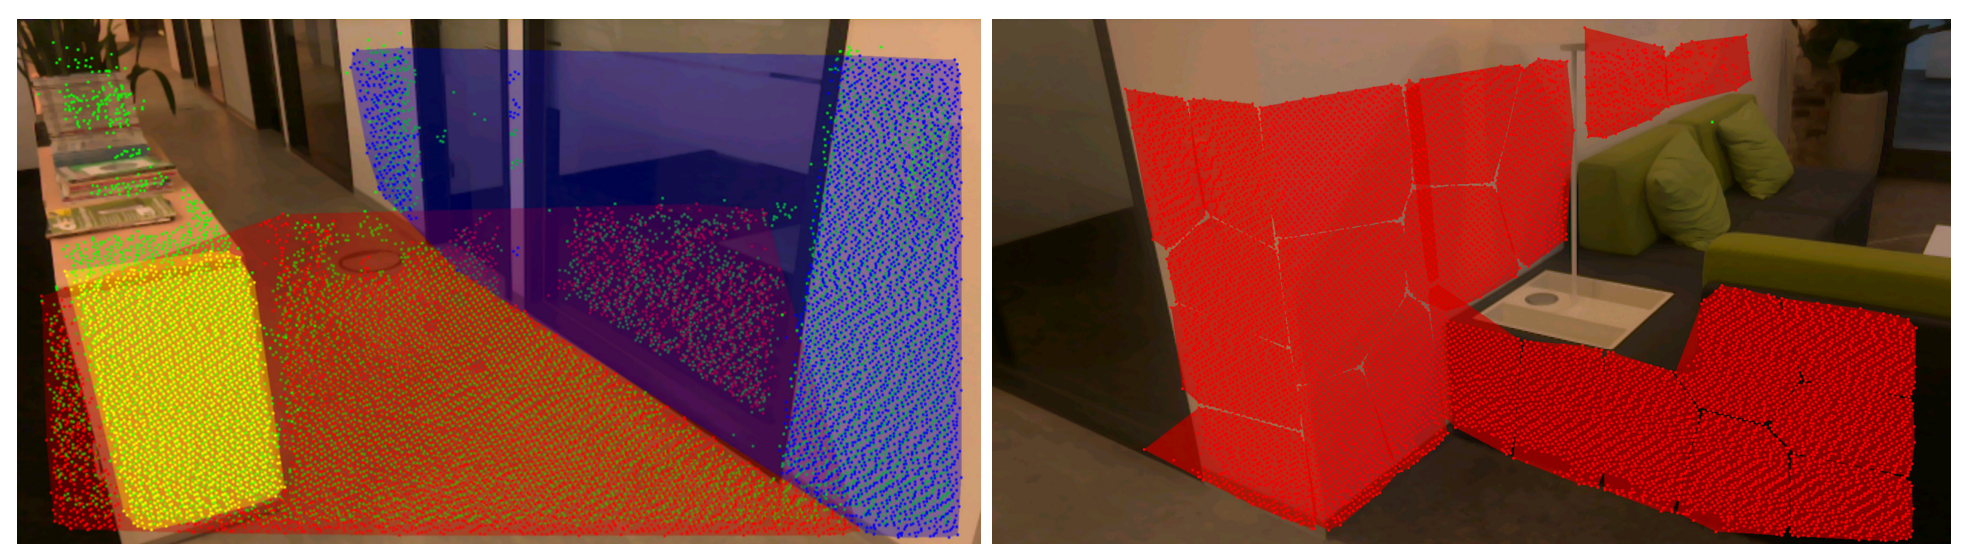
\includegraphics[width=1.0\textwidth]{content/images/methods/clustering.png} 
  \caption{Links: Ebenen Rekonstruktion ohne Clustering. Rechts: Rekonstruktion mit K-Mean Clustering.}
  \label{fig:clustering}
\end{figure}

Getestet wurden hier das K-Mean Clustering, Agglomeratives Clustering und einfaches räumliches Clustern mit Hilfe eines Octrees. Das K-Mean Clustering hat, wie in Abbildung \ref{fig:clustering} rechts zu erkennen, gute Ergebnisse für die Aufteilung einer Ebenen geliefert, benötigt aber zuvor eine feste Anzahl von Clustern. Agglomeratives Clustering, getestet mit dem euklidischen Distanzmaß, würde zwar die Anzahl der Cluster dynamisch bestimmen, ist jedoch zu aufwändig für eine Echtzeit Anwendung, wenn dieser auf die alle Messergebnisse durchgeführt wird. 

Gute Ergebnisse liefert wiederum ein einfaches räumliches Clustern mit einem Octree, welcher die aufgenommenen Punkte direkt in Knoten des Baums zuweist. Das bietet zudem den Vorteil, dass diese Datenstruktur direkt als Speicherort der Aufgenommenen Punkte und Ebenen dienen kann. Außerdem entspricht dies dem Vorgehen für die Anwendung von RANSAC auf Würfeln, welches von \citet{yang2010plane} beschrieben wurde. 
